% \VignetteIndexEntry{goProfiles Vignette}
% \VignetteDepends{Biobase,tools}
% \VignetteKeywords{Gene Ontology Analysis, Microarrays, Gene Set Analysis}
% \VignettePackage{goProfiles}

%\SweaveOpts{prefix.string=images/fig}

\documentclass[a4paper]{article}

\textwidth=6.2in
\textheight=8.5in
%\parskip=.3cm
\oddsidemargin=.1in
\evensidemargin=.1in
\headheight=-.3in


\usepackage{Sweave}
\usepackage{a4wide}
\usepackage{hyperref}
\usepackage{framed}
\usepackage{longtable}
\usepackage{amsmath}
\usepackage{amsfonts}
\usepackage{amssymb}

\usepackage[english]{babel}
\usepackage{times}
\usepackage[T1]{fontenc}

\newcommand{\GO}{\texttt{GO}}
\newcommand{\R}{\texttt{R}}
\newcommand{\Robject}[1]{{\texttt{#1}}}
\newcommand{\Rfunction}[1]{{\texttt{#1}}}
\newcommand{\Rpackage}[1]{{\textit{#1}}}
\newcommand{\Robj}[1]{{\texttt{#1}}}
\newcommand{\Rfun}[1]{{\texttt{#1}}}
\newcommand{\Rpac}[1]{{\textit{#1}}}
\newcommand{\etal}{{\emph et al.}\ }
\newcommand{\etalf}{{\emph et al.}}
\newcommand{\cinlaw}{\buildrel  { \cal L } \over {\small \buildrel \longrightarrow  \over {n \rightarrow \infty}}}
\newcommand{\Prof}{{\mathbf P}}
\newcommand{\rank}{{\rm rank}}
\newtheorem{theorem}{Theorem}[section]


\title{\Rfunction{goProfiles}: an \R\, package for the\\ Statistical Analysis of Functional Profiles}
\author{Alex S\'anchez, Jordi Oca\~na and Miquel Salicr\'u}


\begin{document}

\maketitle



\section{Introduction\label{chap:introduction}}

This document presents an introduction to the use of \Rpackage{goProfiles}, an \R\, package 
for the analysis of lists of genes based on their projection at a given level of the Gene Ontology following the methodology developed by 
\cite{Sanchez:2007a,Salicru:2011}.


\section{Requirements}

To use the package one must have \R\, (2.7 or greater) installed. 
Bioconductor 2.2 or greater is also needed.

\section{Quick start}

For the impatient user the following lines provide a quick and simple
example on the use of the package to explore and compare two
experimental datasets obtained from two prostate cancer experiments
(\cite{Welsh:2001,Singh:2002}). Detailed explanations about the
computations can be found in the following chapters and in the package
help.

The analysis proceeds as follows: 
\begin{itemize}
\item First a dataset is loaded into memory. This dataset contains several lists of genes, from two different studies, 
selected as being differentially expressed in prostate cancer. \Rfunction{help(prostateIds)} will provide extra information about the lists of genes.
\begin{Schunk}
\begin{Sinput}
> require(goProfiles)
> data(prostateIds)
\end{Sinput}
\end{Schunk}
\item Next a functional profile is build for each list. For simplicity it is build for the MF ontology only.
\begin{Schunk}
\begin{Sinput}
> welsh.MF <- basicProfile (welsh01EntrezIDs[1:100], onto="MF", level=2, orgPackage="org.Hs.eg.db") 
> singh.MF <- basicProfile (singh01EntrezIDs[1:100], onto="MF", level=2, orgPackage="org.Hs.eg.db") 
> welsh.singh.MF <-mergeProfilesLists(welsh.MF, singh.MF, profNames=c("Welsh", "Singh"))
> printProfiles(welsh.singh.MF, percentage=TRUE)
\end{Sinput}
\begin{Soutput}
Functional Profile
==================
[1] "MF ontology"
                    Description       GOID Welsh Singh
13         antioxidant activity GO:0016209   1.0   2.1
9                       binding GO:0005488  94.8  91.7
4            catalytic activity GO:0003824  25.8  41.7
18   chemorepellent activity... GO:0045499   0.0   1.0
20 molecular function regula... GO:0098772  13.4  11.5
19 molecular transducer acti... GO:0060089   8.2   5.2
3  nucleic acid binding tran... GO:0001071   5.2   4.2
5  signal transducer activit... GO:0004871  10.3   5.2
7  structural molecule activ... GO:0005198  16.5  15.6
2  transcription factor acti... GO:0000988   2.1   0.0
8          transporter activity GO:0005215   9.3  11.5
\end{Soutput}
\end{Schunk}
\begin{figure}[htbp]
\begin{center}
\begin{Schunk}
\begin{Sinput}
> plotProfiles (welsh.MF, aTitle="Welsh (2001). Prostate cancer data")
\end{Sinput}
\end{Schunk}
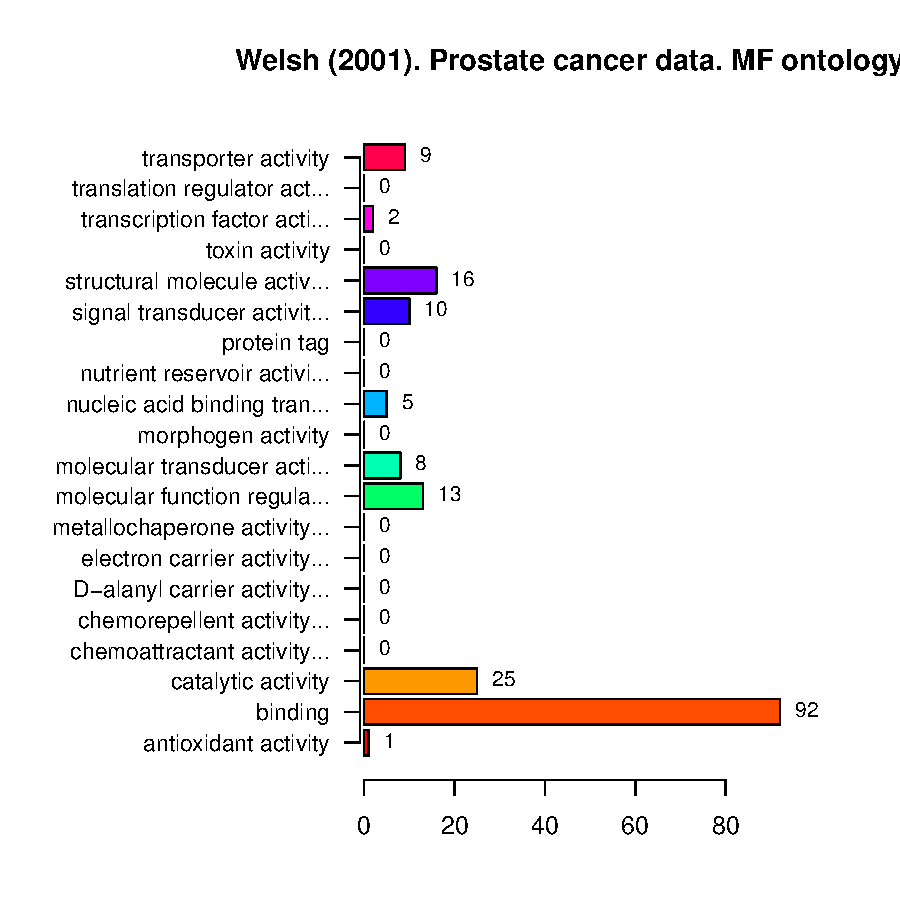
\includegraphics{goProfiles-plotProfileMF}
\end{center}
\caption{\label{welshMF} Basic profile for a dataset at the second level of the MF ontology}
\end{figure}
Changing the parameter \Robj{onto} to '\Robj{ANY}' instead of '\Robj{MF}' will compute profiles for the three ontologies.
\begin{Schunk}
\begin{Sinput}
> welsh <- basicProfile (welsh01EntrezIDs[1:100], onto="ANY", level=2, orgPackage="org.Hs.eg.db") 
\end{Sinput}
\end{Schunk}
\item A visual comparison of profiles can be useful to give hints about the difference between them.
\begin{figure}[htbp]
\begin{center}
\begin{Schunk}
\begin{Sinput}
> plotProfiles (welsh.singh.MF, percentage=T,aTitle="Welsh vs Singh", legend=T) 
\end{Sinput}
\end{Schunk}
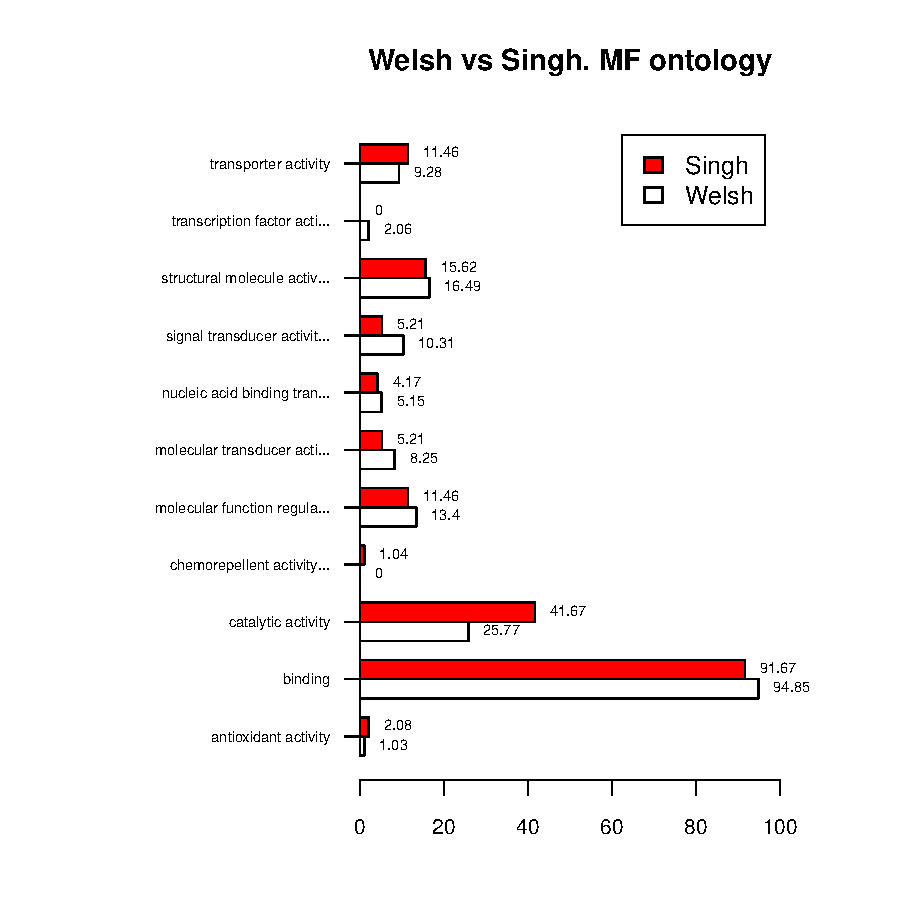
\includegraphics{goProfiles-comparevisual}
\caption{\label{welsh.singh.MF} Comparison between two profiles at the second level of the MF ontology}
\end{center}
\end{figure}
\item Finally a numerical comparison of both profiles is performed and its summary is printed.
Notice that the comparison rebuilds the profiles, that is the input for the computation
are the two lists of genes not the profiles.
\begin{Schunk}
\begin{Sinput}
> compared.welsh.singh.01.MF <- compareGeneLists (welsh01EntrezIDs[1:100], singh01EntrezIDs[1:100], onto="MF", level=2, orgPackage="org.Hs.eg.db")
> print(compSummary(compared.welsh.singh.01.MF))
\end{Sinput}
\begin{Soutput}
Sqr.Euc.Dist       StdErr       pValue   0.95CI.low 
    0.032133     0.022006     0.054600    -0.010998 
   0.95CI.up 
    0.075264 
\end{Soutput}
\end{Schunk}
\item If one finds that the lists are globally different it may be interesting to check out to which categories may be this difference attributed. 
Recent versions of \emph{goProfiles} (from 1.11.02) allow to do a Fisher test on every category in the level of the profile.
\begin{Schunk}
\begin{Sinput}
> list1 <- welsh01EntrezIDs[1:100]
> list2 <- singh01EntrezIDs[1:100]
> commProf <- basicProfile(intersect(list1, list2), onto="MF", level=2, orgPackage="org.Hs.eg.db")$MF
> fisherGOProfiles(welsh.MF$MF, singh.MF$MF, commProf, method="holm")
\end{Sinput}
\begin{Soutput}
GO:0016209 GO:0005488 GO:0003824 GO:0045499 GO:0098772 
   1.00000    1.00000    0.22642    1.00000    1.00000 
GO:0060089 GO:0001071 GO:0004871 GO:0005198 GO:0000988 
   1.00000    1.00000    1.00000    1.00000    1.00000 
GO:0005215 
   1.00000 
attr(,"unadjusted")
GO:0016209 GO:0005488 GO:0003824 GO:0045499 GO:0098772 
  0.497671   0.373836   0.020583   1.000000   1.000000 
GO:0060089 GO:0001071 GO:0004871 GO:0005198 GO:0000988 
  0.559674   0.742220   0.182086   0.839842   0.235467 
GO:0005215 
  0.631968 
\end{Soutput}
\end{Schunk}
\item The reason to compare two lists from similar studies may be to combine them. 
In this case what is more meaningful to do is an equivalence test, instead of a difference test as above.
\begin{Schunk}
\begin{Sinput}
> data(prostateIds)
> expandedWelsh <- expandedProfile(welsh01EntrezIDs[1:100], onto="MF",
+                         level=2, orgPackage="org.Hs.eg.db")
> expandedSingh <- expandedProfile(singh01EntrezIDs[1:100], onto="MF",
+                         level=2, orgPackage="org.Hs.eg.db")
> commonGenes <- intersect(welsh01EntrezIDs[1:100], singh01EntrezIDs[1:100])
> commonExpanded <- expandedProfile(commonGenes, onto="MF", level=2, orgPackage="org.Hs.eg.db")
> equivMF <-equivalentGOProfiles (expandedWelsh[['MF']], 
+                           qm  = expandedSingh[['MF']], 
+                           pqn0= commonExpanded[['MF']])
> print(equivSummary(equivMF, decs=5))
\end{Sinput}
\begin{Soutput}
             Sqr.Euc.Dist                    StdErr 
                  0.03213                   0.02201 
                   pValue                     CI.up 
                  0.58337                   0.06833 
                       d0 Equivalent? (1=yes,0=not) 
                  0.02750                   0.00000 
\end{Soutput}
\begin{Sinput}
> 
\end{Sinput}
\end{Schunk}
\end{itemize}


\section{User guide}

This introduction has simply shown the possibilities of the program. A more complete user guide can be found at the program's web site:\newline \href{http://estbioinfo.stat.ub.es/pubs/goProfiles-Usersguide.pdf}{http://estbioinfo.stat.ub.es/pubs/goProfiles-Usersguide.pdf}

\bibliographystyle{plain}

\addcontentsline{toc}{section}{\refname}
%\bibliography{references-goProfiles}
\begin{thebibliography}{10}


\bibitem{Singh:2002}
Singh, Dinesh., William~R Sellers, Philip~K. Febbo, Kenneth Ross, Donald~G
  Jackson, Judith Manola, Christine Ladd, Pablo Tamayo, Andrew~A Renshaw,
  Anthony~V D'Amico, Jerome~P Richie, Eric~S Lander, Massimo Loda, Philip~W
  Kantoff, and Todd~R Golub.
\newblock Gene expression correlates of clinical prostate cancer behavior.
\newblock {\em Cancer Cell}, 1(2):203--209, 2002.

\bibitem{Sanchez:2007a}
A.~S{\'a}nchez-Pla, M.~Salicr{\'u}, and J.~Oca{\~n}a.
\newblock Statistical methods for the analysis of high-throughput data based on
  functional profiles derived from the gene ontology.
\newblock {\em Journal of Statistical Planning and Inference}, 137(12):3975--3989, 2007. 

\bibitem{Salicru:2011}
  M. Salicr{\'u}, J. Oca{\~n}a and A. S{\'a}nchez-Pla.
\newblock Comparison of Gene Lists based on Functional Profiles.
\newblock {\em BMC Bioinformatics}, DOI: 10.1186/1471-2105-12-401, 2011.

\bibitem{Welsh:2001}
J.B. Welsh, Lisa~M. Sapinoso, Andrew~I. Su, Suzanne~G. Kern, Jessica
  Wang-Rodriguez, Christopher~A. Moskaluk-Jr., Henry~F. Frierson, and
  Hampton~Garret M.
\newblock Analysis of gene expression identifies candidate markers and
  pharmacological targets in prostate cancer.
\newblock {\em Cancer Res}, 61:5974--5978, 2001.

\end{thebibliography}


\end{document}

